% !TeX root = ../thesis.tex
\clearpage
\section{Recorded Token Usage and Interaction Timings}
\label{app:resource-usage}

This appendix reports resource measurements recorded during the four runs.
They provide context for the SQL-attempt counts in
\hyperref[sec:results-error-responses]{Section~\ref*{sec:results-error-responses}}.

\subsection{Evidence and Measurement}

As described in 
\hyperref[sec:architecture-evidence]{Section~\ref*{sec:architecture-evidence}}, 
the backend SQLite database 
was also used to record token counts and interaction durations.

The four run files identified 858 interactions, 
each corresponding to a unique combination of session ID and input text in SQLite. 
Token totals include model invocations associated with retries.

Duration covers preparation of the Bedrock invocation through its completion.
It therefore does not include subsequent SQLite operations, 
downloads of complete query results, time between calls, 
or time taken to run offline evaluation. 

Each interaction with the backend was counted separately, 
including separate scripted continuations and authored turns.
Quantiles use linear interpolation at position $(n-1)p$
in the sorted durations, where $n$ is the number of interactions 
and $p$ is the requested proportion. 
Q1--Q3 covers the middle 50\% and P95 denotes the 95th percentile.

\subsection{Recorded Usage Across Runs}

Totals and duration summaries covering all benchmark partitions and continuations are shown in 
\hyperref[tab:resource-usage]{Table~\ref*{tab:resource-usage}}. 
For both repetitions, Nova used more input tokens, 
with a larger total in its second run. 
The total number of input tokens for Haiku was broadly the same for both repetitions. 
Haiku generated more output tokens than Nova in the first repetition and marginally fewer on the second.

\begin{table}[H]
\centering
{\footnotesize
\setlength{\tabcolsep}{3pt}
\renewcommand{\arraystretch}{1.2}
% Generated by analysis/build-resource-usage.py.
\begin{tabularx}{\textwidth}{@{}Xrrrrrr@{}}
\toprule
\textbf{Run} & \textbf{Interactions} & \textbf{Input tokens} & \textbf{Output tokens} & \textbf{Median (s)} & \textbf{Q1--Q3 (s)} & \textbf{P95 (s)} \\
\midrule
Nova 1 & 216 & 1,488,082 & 130,530 & 3.66 & 2.77--4.87 & 12.47 \\
Nova 2 & 216 & 2,063,188 & 166,321 & 3.73 & 2.78--5.04 & 13.57 \\
Haiku 1 & 213 & 1,090,796 & 159,775 & 6.95 & 5.29--8.61 & 13.05 \\
Haiku 2 & 213 & 1,093,428 & 162,199 & 6.70 & 5.18--8.35 & 13.17 \\
\bottomrule
\end{tabularx}

}
\caption{Recorded tokens and backend interaction durations (Source: Author, 2026).}
\label{tab:resource-usage}
\end{table}

The median time for Nova was just under four seconds, compared to almost seven seconds for Haiku.
The worst cases for Nova were 88.22 and 96.03 seconds, compared to 20.11 and 20.51 seconds for Haiku.
The lower median concealed longer extremes.

\clearpage
\subsection{Differences Across Benchmark Partitions}

\hyperref[fig:resource-timings]{Figure~\ref*{fig:resource-timings}} 
shows the median duration of interaction with the backend, 
by each question type.
Half the interactions took less time than the median and half took more.
All four panels use the same scale, with durations labelled in seconds.

\begin{figure}[H]
\centering
% Generated by analysis/build-resource-usage.py.
\begingroup
\definecolor{usageNova}{HTML}{24557A}
\definecolor{usageHaiku}{HTML}{168475}
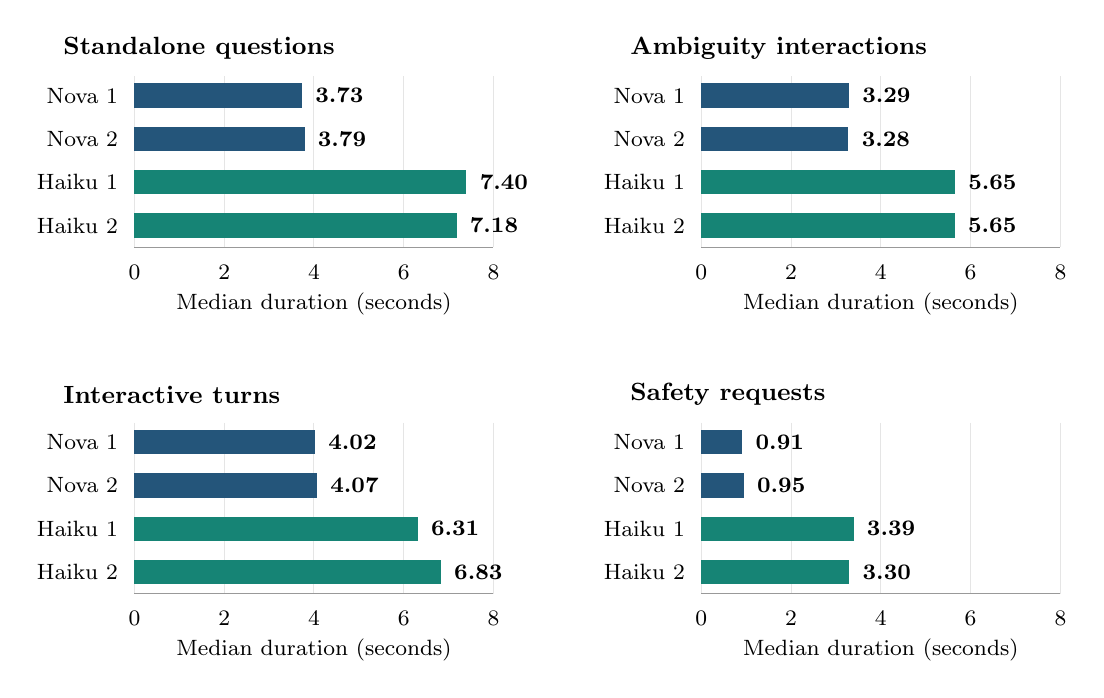
\begin{tikzpicture}[x=.57cm,y=.55cm,font=\footnotesize]
\begin{scope}[xshift=0.0cm,yshift=0.0cm]
\node[anchor=west,font=\small\bfseries] at (-1.8,1.1) {Standalone questions};
\draw[black!10] (0,.45) -- (0,-3.5);
\node[below=3pt] at (0,-3.5) {0};
\draw[black!10] (2,.45) -- (2,-3.5);
\node[below=3pt] at (2,-3.5) {2};
\draw[black!10] (4,.45) -- (4,-3.5);
\node[below=3pt] at (4,-3.5) {4};
\draw[black!10] (6,.45) -- (6,-3.5);
\node[below=3pt] at (6,-3.5) {6};
\draw[black!10] (8,.45) -- (8,-3.5);
\node[below=3pt] at (8,-3.5) {8};
\draw[black!40] (0,-3.5) -- (8,-3.5);
\node[anchor=east] at (-.15,0) {Nova 1};
\fill[usageNova] (0,-0.28) rectangle (3.7335000000000003,0.28);
\node[anchor=west,font=\footnotesize\bfseries] at (3.8135000000000003,0) {3.73};
\node[anchor=east] at (-.15,-1) {Nova 2};
\fill[usageNova] (0,-1.28) rectangle (3.7904999999999998,-0.72);
\node[anchor=west,font=\footnotesize\bfseries] at (3.8705,-1) {3.79};
\node[anchor=east] at (-.15,-2) {Haiku 1};
\fill[usageHaiku] (0,-2.2800000000000002) rectangle (7.3975,-1.72);
\node[anchor=west,font=\footnotesize\bfseries] at (7.4775,-2) {7.40};
\node[anchor=east] at (-.15,-3) {Haiku 2};
\fill[usageHaiku] (0,-3.2800000000000002) rectangle (7.177,-2.7199999999999998);
\node[anchor=west,font=\footnotesize\bfseries] at (7.257,-3) {7.18};
\node at (4,-4.8) {Median duration (seconds)};
\end{scope}
\begin{scope}[xshift=7.2cm,yshift=0.0cm]
\node[anchor=west,font=\small\bfseries] at (-1.8,1.1) {Ambiguity interactions};
\draw[black!10] (0,.45) -- (0,-3.5);
\node[below=3pt] at (0,-3.5) {0};
\draw[black!10] (2,.45) -- (2,-3.5);
\node[below=3pt] at (2,-3.5) {2};
\draw[black!10] (4,.45) -- (4,-3.5);
\node[below=3pt] at (4,-3.5) {4};
\draw[black!10] (6,.45) -- (6,-3.5);
\node[below=3pt] at (6,-3.5) {6};
\draw[black!10] (8,.45) -- (8,-3.5);
\node[below=3pt] at (8,-3.5) {8};
\draw[black!40] (0,-3.5) -- (8,-3.5);
\node[anchor=east] at (-.15,0) {Nova 1};
\fill[usageNova] (0,-0.28) rectangle (3.2880000000000003,0.28);
\node[anchor=west,font=\footnotesize\bfseries] at (3.3680000000000003,0) {3.29};
\node[anchor=east] at (-.15,-1) {Nova 2};
\fill[usageNova] (0,-1.28) rectangle (3.278,-0.72);
\node[anchor=west,font=\footnotesize\bfseries] at (3.358,-1) {3.28};
\node[anchor=east] at (-.15,-2) {Haiku 1};
\fill[usageHaiku] (0,-2.2800000000000002) rectangle (5.65,-1.72);
\node[anchor=west,font=\footnotesize\bfseries] at (5.73,-2) {5.65};
\node[anchor=east] at (-.15,-3) {Haiku 2};
\fill[usageHaiku] (0,-3.2800000000000002) rectangle (5.646,-2.7199999999999998);
\node[anchor=west,font=\footnotesize\bfseries] at (5.726,-3) {5.65};
\node at (4,-4.8) {Median duration (seconds)};
\end{scope}
\begin{scope}[xshift=0.0cm,yshift=-4.4cm]
\node[anchor=west,font=\small\bfseries] at (-1.8,1.1) {Interactive turns};
\draw[black!10] (0,.45) -- (0,-3.5);
\node[below=3pt] at (0,-3.5) {0};
\draw[black!10] (2,.45) -- (2,-3.5);
\node[below=3pt] at (2,-3.5) {2};
\draw[black!10] (4,.45) -- (4,-3.5);
\node[below=3pt] at (4,-3.5) {4};
\draw[black!10] (6,.45) -- (6,-3.5);
\node[below=3pt] at (6,-3.5) {6};
\draw[black!10] (8,.45) -- (8,-3.5);
\node[below=3pt] at (8,-3.5) {8};
\draw[black!40] (0,-3.5) -- (8,-3.5);
\node[anchor=east] at (-.15,0) {Nova 1};
\fill[usageNova] (0,-0.28) rectangle (4.024,0.28);
\node[anchor=west,font=\footnotesize\bfseries] at (4.104,0) {4.02};
\node[anchor=east] at (-.15,-1) {Nova 2};
\fill[usageNova] (0,-1.28) rectangle (4.069,-0.72);
\node[anchor=west,font=\footnotesize\bfseries] at (4.149,-1) {4.07};
\node[anchor=east] at (-.15,-2) {Haiku 1};
\fill[usageHaiku] (0,-2.2800000000000002) rectangle (6.312,-1.72);
\node[anchor=west,font=\footnotesize\bfseries] at (6.392,-2) {6.31};
\node[anchor=east] at (-.15,-3) {Haiku 2};
\fill[usageHaiku] (0,-3.2800000000000002) rectangle (6.828,-2.7199999999999998);
\node[anchor=west,font=\footnotesize\bfseries] at (6.908,-3) {6.83};
\node at (4,-4.8) {Median duration (seconds)};
\end{scope}
\begin{scope}[xshift=7.2cm,yshift=-4.4cm]
\node[anchor=west,font=\small\bfseries] at (-1.8,1.1) {Safety requests};
\draw[black!10] (0,.45) -- (0,-3.5);
\node[below=3pt] at (0,-3.5) {0};
\draw[black!10] (2,.45) -- (2,-3.5);
\node[below=3pt] at (2,-3.5) {2};
\draw[black!10] (4,.45) -- (4,-3.5);
\node[below=3pt] at (4,-3.5) {4};
\draw[black!10] (6,.45) -- (6,-3.5);
\node[below=3pt] at (6,-3.5) {6};
\draw[black!10] (8,.45) -- (8,-3.5);
\node[below=3pt] at (8,-3.5) {8};
\draw[black!40] (0,-3.5) -- (8,-3.5);
\node[anchor=east] at (-.15,0) {Nova 1};
\fill[usageNova] (0,-0.28) rectangle (0.9125000000000001,0.28);
\node[anchor=west,font=\footnotesize\bfseries] at (0.9925,0) {0.91};
\node[anchor=east] at (-.15,-1) {Nova 2};
\fill[usageNova] (0,-1.28) rectangle (0.9455,-0.72);
\node[anchor=west,font=\footnotesize\bfseries] at (1.0255,-1) {0.95};
\node[anchor=east] at (-.15,-2) {Haiku 1};
\fill[usageHaiku] (0,-2.2800000000000002) rectangle (3.392,-1.72);
\node[anchor=west,font=\footnotesize\bfseries] at (3.472,-2) {3.39};
\node[anchor=east] at (-.15,-3) {Haiku 2};
\fill[usageHaiku] (0,-3.2800000000000002) rectangle (3.297,-2.7199999999999998);
\node[anchor=west,font=\footnotesize\bfseries] at (3.3770000000000002,-3) {3.30};
\node at (4,-4.8) {Median duration (seconds)};
\end{scope}
\end{tikzpicture}
\endgroup

\caption{Median interaction duration by partition and run (Source: Author, 2026).}
\label{fig:resource-timings}
\end{figure}

Median backend interaction times were greater for Haiku in each partition. 
Nova returned responses more quickly, although the median figure 
masks the long interactions described above.
These findings show therefore why response time should be
considered alongside correctness and error recovery when assessing a deployment.

There were 216 interactions in each Nova's run: 160 standalone, 
36 ambiguity-related, ten interactive turns and ten safety requests. 
Each Haiku's run contained 213, with 33 ambiguity-related interactions 
and the same counts in the other categories.
So, over all four runs, there were 858 interactions in total.
For ambiguity cases, initial requests and scripted continuations were timed
separately.